% Options for packages loaded elsewhere
\PassOptionsToPackage{unicode}{hyperref}
\PassOptionsToPackage{hyphens}{url}
\PassOptionsToPackage{dvipsnames,svgnames,x11names}{xcolor}
%
\documentclass[
  letterpaper,
  DIV=11,
  numbers=noendperiod]{scrartcl}

\usepackage{amsmath,amssymb}
\usepackage{iftex}
\ifPDFTeX
  \usepackage[T1]{fontenc}
  \usepackage[utf8]{inputenc}
  \usepackage{textcomp} % provide euro and other symbols
\else % if luatex or xetex
  \usepackage{unicode-math}
  \defaultfontfeatures{Scale=MatchLowercase}
  \defaultfontfeatures[\rmfamily]{Ligatures=TeX,Scale=1}
\fi
\usepackage{lmodern}
\ifPDFTeX\else  
    % xetex/luatex font selection
\fi
% Use upquote if available, for straight quotes in verbatim environments
\IfFileExists{upquote.sty}{\usepackage{upquote}}{}
\IfFileExists{microtype.sty}{% use microtype if available
  \usepackage[]{microtype}
  \UseMicrotypeSet[protrusion]{basicmath} % disable protrusion for tt fonts
}{}
\makeatletter
\@ifundefined{KOMAClassName}{% if non-KOMA class
  \IfFileExists{parskip.sty}{%
    \usepackage{parskip}
  }{% else
    \setlength{\parindent}{0pt}
    \setlength{\parskip}{6pt plus 2pt minus 1pt}}
}{% if KOMA class
  \KOMAoptions{parskip=half}}
\makeatother
\usepackage{xcolor}
\setlength{\emergencystretch}{3em} % prevent overfull lines
\setcounter{secnumdepth}{-\maxdimen} % remove section numbering
% Make \paragraph and \subparagraph free-standing
\makeatletter
\ifx\paragraph\undefined\else
  \let\oldparagraph\paragraph
  \renewcommand{\paragraph}{
    \@ifstar
      \xxxParagraphStar
      \xxxParagraphNoStar
  }
  \newcommand{\xxxParagraphStar}[1]{\oldparagraph*{#1}\mbox{}}
  \newcommand{\xxxParagraphNoStar}[1]{\oldparagraph{#1}\mbox{}}
\fi
\ifx\subparagraph\undefined\else
  \let\oldsubparagraph\subparagraph
  \renewcommand{\subparagraph}{
    \@ifstar
      \xxxSubParagraphStar
      \xxxSubParagraphNoStar
  }
  \newcommand{\xxxSubParagraphStar}[1]{\oldsubparagraph*{#1}\mbox{}}
  \newcommand{\xxxSubParagraphNoStar}[1]{\oldsubparagraph{#1}\mbox{}}
\fi
\makeatother

\usepackage{color}
\usepackage{fancyvrb}
\newcommand{\VerbBar}{|}
\newcommand{\VERB}{\Verb[commandchars=\\\{\}]}
\DefineVerbatimEnvironment{Highlighting}{Verbatim}{commandchars=\\\{\}}
% Add ',fontsize=\small' for more characters per line
\usepackage{framed}
\definecolor{shadecolor}{RGB}{241,243,245}
\newenvironment{Shaded}{\begin{snugshade}}{\end{snugshade}}
\newcommand{\AlertTok}[1]{\textcolor[rgb]{0.68,0.00,0.00}{#1}}
\newcommand{\AnnotationTok}[1]{\textcolor[rgb]{0.37,0.37,0.37}{#1}}
\newcommand{\AttributeTok}[1]{\textcolor[rgb]{0.40,0.45,0.13}{#1}}
\newcommand{\BaseNTok}[1]{\textcolor[rgb]{0.68,0.00,0.00}{#1}}
\newcommand{\BuiltInTok}[1]{\textcolor[rgb]{0.00,0.23,0.31}{#1}}
\newcommand{\CharTok}[1]{\textcolor[rgb]{0.13,0.47,0.30}{#1}}
\newcommand{\CommentTok}[1]{\textcolor[rgb]{0.37,0.37,0.37}{#1}}
\newcommand{\CommentVarTok}[1]{\textcolor[rgb]{0.37,0.37,0.37}{\textit{#1}}}
\newcommand{\ConstantTok}[1]{\textcolor[rgb]{0.56,0.35,0.01}{#1}}
\newcommand{\ControlFlowTok}[1]{\textcolor[rgb]{0.00,0.23,0.31}{\textbf{#1}}}
\newcommand{\DataTypeTok}[1]{\textcolor[rgb]{0.68,0.00,0.00}{#1}}
\newcommand{\DecValTok}[1]{\textcolor[rgb]{0.68,0.00,0.00}{#1}}
\newcommand{\DocumentationTok}[1]{\textcolor[rgb]{0.37,0.37,0.37}{\textit{#1}}}
\newcommand{\ErrorTok}[1]{\textcolor[rgb]{0.68,0.00,0.00}{#1}}
\newcommand{\ExtensionTok}[1]{\textcolor[rgb]{0.00,0.23,0.31}{#1}}
\newcommand{\FloatTok}[1]{\textcolor[rgb]{0.68,0.00,0.00}{#1}}
\newcommand{\FunctionTok}[1]{\textcolor[rgb]{0.28,0.35,0.67}{#1}}
\newcommand{\ImportTok}[1]{\textcolor[rgb]{0.00,0.46,0.62}{#1}}
\newcommand{\InformationTok}[1]{\textcolor[rgb]{0.37,0.37,0.37}{#1}}
\newcommand{\KeywordTok}[1]{\textcolor[rgb]{0.00,0.23,0.31}{\textbf{#1}}}
\newcommand{\NormalTok}[1]{\textcolor[rgb]{0.00,0.23,0.31}{#1}}
\newcommand{\OperatorTok}[1]{\textcolor[rgb]{0.37,0.37,0.37}{#1}}
\newcommand{\OtherTok}[1]{\textcolor[rgb]{0.00,0.23,0.31}{#1}}
\newcommand{\PreprocessorTok}[1]{\textcolor[rgb]{0.68,0.00,0.00}{#1}}
\newcommand{\RegionMarkerTok}[1]{\textcolor[rgb]{0.00,0.23,0.31}{#1}}
\newcommand{\SpecialCharTok}[1]{\textcolor[rgb]{0.37,0.37,0.37}{#1}}
\newcommand{\SpecialStringTok}[1]{\textcolor[rgb]{0.13,0.47,0.30}{#1}}
\newcommand{\StringTok}[1]{\textcolor[rgb]{0.13,0.47,0.30}{#1}}
\newcommand{\VariableTok}[1]{\textcolor[rgb]{0.07,0.07,0.07}{#1}}
\newcommand{\VerbatimStringTok}[1]{\textcolor[rgb]{0.13,0.47,0.30}{#1}}
\newcommand{\WarningTok}[1]{\textcolor[rgb]{0.37,0.37,0.37}{\textit{#1}}}

\providecommand{\tightlist}{%
  \setlength{\itemsep}{0pt}\setlength{\parskip}{0pt}}\usepackage{longtable,booktabs,array}
\usepackage{calc} % for calculating minipage widths
% Correct order of tables after \paragraph or \subparagraph
\usepackage{etoolbox}
\makeatletter
\patchcmd\longtable{\par}{\if@noskipsec\mbox{}\fi\par}{}{}
\makeatother
% Allow footnotes in longtable head/foot
\IfFileExists{footnotehyper.sty}{\usepackage{footnotehyper}}{\usepackage{footnote}}
\makesavenoteenv{longtable}
\usepackage{graphicx}
\makeatletter
\def\maxwidth{\ifdim\Gin@nat@width>\linewidth\linewidth\else\Gin@nat@width\fi}
\def\maxheight{\ifdim\Gin@nat@height>\textheight\textheight\else\Gin@nat@height\fi}
\makeatother
% Scale images if necessary, so that they will not overflow the page
% margins by default, and it is still possible to overwrite the defaults
% using explicit options in \includegraphics[width, height, ...]{}
\setkeys{Gin}{width=\maxwidth,height=\maxheight,keepaspectratio}
% Set default figure placement to htbp
\makeatletter
\def\fps@figure{htbp}
\makeatother

\KOMAoption{captions}{tableheading}
\makeatletter
\@ifpackageloaded{caption}{}{\usepackage{caption}}
\AtBeginDocument{%
\ifdefined\contentsname
  \renewcommand*\contentsname{Tabla de contenidos}
\else
  \newcommand\contentsname{Tabla de contenidos}
\fi
\ifdefined\listfigurename
  \renewcommand*\listfigurename{Listado de Figuras}
\else
  \newcommand\listfigurename{Listado de Figuras}
\fi
\ifdefined\listtablename
  \renewcommand*\listtablename{Listado de Tablas}
\else
  \newcommand\listtablename{Listado de Tablas}
\fi
\ifdefined\figurename
  \renewcommand*\figurename{Figura}
\else
  \newcommand\figurename{Figura}
\fi
\ifdefined\tablename
  \renewcommand*\tablename{Tabla}
\else
  \newcommand\tablename{Tabla}
\fi
}
\@ifpackageloaded{float}{}{\usepackage{float}}
\floatstyle{ruled}
\@ifundefined{c@chapter}{\newfloat{codelisting}{h}{lop}}{\newfloat{codelisting}{h}{lop}[chapter]}
\floatname{codelisting}{Listado}
\newcommand*\listoflistings{\listof{codelisting}{Listado de Listados}}
\makeatother
\makeatletter
\makeatother
\makeatletter
\@ifpackageloaded{caption}{}{\usepackage{caption}}
\@ifpackageloaded{subcaption}{}{\usepackage{subcaption}}
\makeatother

\ifLuaTeX
\usepackage[bidi=basic]{babel}
\else
\usepackage[bidi=default]{babel}
\fi
\babelprovide[main,import]{spanish}
% get rid of language-specific shorthands (see #6817):
\let\LanguageShortHands\languageshorthands
\def\languageshorthands#1{}
\ifLuaTeX
  \usepackage{selnolig}  % disable illegal ligatures
\fi
\usepackage{bookmark}

\IfFileExists{xurl.sty}{\usepackage{xurl}}{} % add URL line breaks if available
\urlstyle{same} % disable monospaced font for URLs
\hypersetup{
  pdftitle={Corrección},
  pdfauthor={Boris Garcés},
  pdflang={es},
  colorlinks=true,
  linkcolor={blue},
  filecolor={Maroon},
  citecolor={Blue},
  urlcolor={Blue},
  pdfcreator={LaTeX via pandoc}}


\title{Corrección}
\author{Boris Garcés}
\date{}

\begin{document}
\maketitle

\renewcommand*\contentsname{Tabla de Contenidos}
{
\hypersetup{linkcolor=}
\setcounter{tocdepth}{3}
\tableofcontents
}

\subsection{Repositorio}\label{repositorio}

https://github.com/Boris-epn/prueba-correccion

\begin{Shaded}
\begin{Highlighting}[]
\OperatorTok{\%}\NormalTok{load\_ext autoreload}
\end{Highlighting}
\end{Shaded}

\section{Examen}\label{examen}

\subsection{Determinante}\label{determinante}

\begin{Shaded}
\begin{Highlighting}[]
\ImportTok{import}\NormalTok{ numpy }\ImportTok{as}\NormalTok{ np}
\ImportTok{from}\NormalTok{ src }\ImportTok{import}\NormalTok{ (}
\NormalTok{    eliminacion\_gaussiana,}
\NormalTok{    descomposicion\_LU,}
\NormalTok{    resolver\_LU,}
\NormalTok{    matriz\_aumentada,}
\NormalTok{    separar\_m\_aumentada,}
\NormalTok{)}

\CommentTok{\# Examen}
\CommentTok{\#\# Determinante}
\KeywordTok{def}\NormalTok{ calc\_determinante(A: }\BuiltInTok{list}\NormalTok{[}\BuiltInTok{list}\NormalTok{[}\BuiltInTok{float}\NormalTok{]]) }\OperatorTok{{-}\textgreater{}} \BuiltInTok{float}\NormalTok{:}
    \CommentTok{"""Función que calcula el determinante usando la descomposición LU.}

\CommentTok{    \#\# Parameters}
\CommentTok{    \textasciigrave{}\textasciigrave{}A\textasciigrave{}\textasciigrave{}: Matriz cuadrada de tamaño n x n}

\CommentTok{    \#\# Return}
\CommentTok{    \textasciigrave{}\textasciigrave{}detA\textasciigrave{}\textasciigrave{}: Determinante de la matriz A}
\CommentTok{    """}
\NormalTok{    A }\OperatorTok{=}\NormalTok{ np.array(A, dtype}\OperatorTok{=}\BuiltInTok{float}\NormalTok{)}
\NormalTok{    L, U }\OperatorTok{=}\NormalTok{ descomposicion\_LU(A)}
\NormalTok{    detA }\OperatorTok{=}\NormalTok{ np.prod(np.diagonal(U))}

    \ControlFlowTok{return}\NormalTok{ detA}
\end{Highlighting}
\end{Shaded}

\section{Ejercicio 1}\label{ejercicio-1}

\begin{Shaded}
\begin{Highlighting}[]
\NormalTok{A1 }\OperatorTok{=}\NormalTok{ [}
\NormalTok{    [}\OperatorTok{{-}}\DecValTok{4}\NormalTok{, }\DecValTok{2}\NormalTok{, }\OperatorTok{{-}}\DecValTok{4}\NormalTok{, }\OperatorTok{{-}}\DecValTok{4}\NormalTok{, }\DecValTok{1}\NormalTok{, }\DecValTok{2}\NormalTok{, }\DecValTok{5}\NormalTok{, }\DecValTok{3}\NormalTok{, }\DecValTok{5}\NormalTok{, }\DecValTok{1}\NormalTok{],}
\NormalTok{    [}\DecValTok{1}\NormalTok{, }\DecValTok{0}\NormalTok{, }\DecValTok{4}\NormalTok{, }\DecValTok{3}\NormalTok{, }\DecValTok{0}\NormalTok{, }\OperatorTok{{-}}\DecValTok{2}\NormalTok{, }\DecValTok{3}\NormalTok{, }\DecValTok{0}\NormalTok{, }\DecValTok{1}\NormalTok{, }\DecValTok{5}\NormalTok{],}
\NormalTok{    [}\DecValTok{5}\NormalTok{, }\DecValTok{5}\NormalTok{, }\OperatorTok{{-}}\DecValTok{4}\NormalTok{, }\DecValTok{5}\NormalTok{, }\OperatorTok{{-}}\DecValTok{4}\NormalTok{, }\DecValTok{2}\NormalTok{, }\DecValTok{2}\NormalTok{, }\DecValTok{2}\NormalTok{, }\DecValTok{4}\NormalTok{, }\DecValTok{4}\NormalTok{],}
\NormalTok{    [}\OperatorTok{{-}}\DecValTok{1}\NormalTok{, }\DecValTok{3}\NormalTok{, }\DecValTok{4}\NormalTok{, }\OperatorTok{{-}}\DecValTok{1}\NormalTok{, }\OperatorTok{{-}}\DecValTok{4}\NormalTok{, }\DecValTok{0}\NormalTok{, }\DecValTok{5}\NormalTok{, }\DecValTok{0}\NormalTok{, }\DecValTok{0}\NormalTok{, }\DecValTok{5}\NormalTok{],}
\NormalTok{    [}\DecValTok{4}\NormalTok{, }\DecValTok{1}\NormalTok{, }\DecValTok{4}\NormalTok{, }\DecValTok{2}\NormalTok{, }\DecValTok{0}\NormalTok{, }\DecValTok{0}\NormalTok{, }\DecValTok{3}\NormalTok{, }\OperatorTok{{-}}\DecValTok{1}\NormalTok{, }\DecValTok{0}\NormalTok{, }\DecValTok{2}\NormalTok{],}
\NormalTok{    [}\DecValTok{2}\NormalTok{, }\OperatorTok{{-}}\DecValTok{2}\NormalTok{, }\DecValTok{1}\NormalTok{, }\OperatorTok{{-}}\DecValTok{1}\NormalTok{, }\OperatorTok{{-}}\DecValTok{2}\NormalTok{, }\OperatorTok{{-}}\DecValTok{3}\NormalTok{, }\DecValTok{2}\NormalTok{, }\OperatorTok{{-}}\DecValTok{2}\NormalTok{, }\DecValTok{4}\NormalTok{, }\OperatorTok{{-}}\DecValTok{1}\NormalTok{],}
\NormalTok{    [}\DecValTok{3}\NormalTok{, }\OperatorTok{{-}}\DecValTok{2}\NormalTok{, }\OperatorTok{{-}}\DecValTok{3}\NormalTok{, }\OperatorTok{{-}}\DecValTok{2}\NormalTok{, }\OperatorTok{{-}}\DecValTok{1}\NormalTok{, }\OperatorTok{{-}}\DecValTok{3}\NormalTok{, }\DecValTok{5}\NormalTok{, }\OperatorTok{{-}}\DecValTok{1}\NormalTok{, }\DecValTok{5}\NormalTok{, }\DecValTok{0}\NormalTok{],}
\NormalTok{    [}\DecValTok{3}\NormalTok{, }\DecValTok{4}\NormalTok{, }\OperatorTok{{-}}\DecValTok{3}\NormalTok{, }\DecValTok{3}\NormalTok{, }\OperatorTok{{-}}\DecValTok{2}\NormalTok{, }\DecValTok{2}\NormalTok{, }\OperatorTok{{-}}\DecValTok{4}\NormalTok{, }\OperatorTok{{-}}\DecValTok{4}\NormalTok{, }\DecValTok{1}\NormalTok{, }\DecValTok{5}\NormalTok{],}
\NormalTok{    [}\OperatorTok{{-}}\DecValTok{4}\NormalTok{, }\DecValTok{0}\NormalTok{, }\DecValTok{3}\NormalTok{, }\DecValTok{3}\NormalTok{, }\OperatorTok{{-}}\DecValTok{3}\NormalTok{, }\OperatorTok{{-}}\DecValTok{2}\NormalTok{, }\OperatorTok{{-}}\DecValTok{2}\NormalTok{, }\DecValTok{0}\NormalTok{, }\DecValTok{5}\NormalTok{, }\OperatorTok{{-}}\DecValTok{4}\NormalTok{],}
\NormalTok{    [}\OperatorTok{{-}}\DecValTok{2}\NormalTok{, }\DecValTok{4}\NormalTok{, }\DecValTok{4}\NormalTok{, }\OperatorTok{{-}}\DecValTok{2}\NormalTok{, }\OperatorTok{{-}}\DecValTok{1}\NormalTok{, }\DecValTok{1}\NormalTok{, }\DecValTok{5}\NormalTok{, }\OperatorTok{{-}}\DecValTok{1}\NormalTok{, }\DecValTok{3}\NormalTok{, }\OperatorTok{{-}}\DecValTok{3}\NormalTok{],}
\NormalTok{]}
\NormalTok{calc\_determinante(A1)}
\end{Highlighting}
\end{Shaded}

\begin{verbatim}
[01-23 11:59:58][INFO] 
[[-4.    2.   -4.   -4.    1.    2.    5.    3.    5.    1.  ]
 [ 0.    0.5   3.    2.    0.25 -1.5   4.25  0.75  2.25  5.25]
 [ 0.    7.5  -9.    0.   -2.75  4.5   8.25  5.75 10.25  5.25]
 [ 0.    2.5   5.    0.   -4.25 -0.5   3.75 -0.75 -1.25  4.75]
 [ 0.    3.    0.   -2.    1.    2.    8.    2.    5.    3.  ]
 [ 0.   -1.   -1.   -3.   -1.5  -2.    4.5  -0.5   6.5  -0.5 ]
 [ 0.   -0.5  -6.   -5.   -0.25 -1.5   8.75  1.25  8.75  0.75]
 [ 0.    5.5  -6.    0.   -1.25  3.5  -0.25 -1.75  4.75  5.75]
 [ 0.   -2.    7.    7.   -4.   -4.   -7.   -3.    0.   -5.  ]
 [ 0.    3.    6.    0.   -1.5   0.    2.5  -2.5   0.5  -3.5 ]]
[01-23 11:59:58][INFO] 
[[ -4.     2.    -4.    -4.     1.     2.     5.     3.     5.     1.  ]
 [  0.     0.5    3.     2.     0.25  -1.5    4.25   0.75   2.25   5.25]
 [  0.     0.   -54.   -30.    -6.5   27.   -55.5   -5.5  -23.5  -73.5 ]
 [  0.     0.   -10.   -10.    -5.5    7.   -17.5   -4.5  -12.5  -21.5 ]
 [  0.     0.   -18.   -14.    -0.5   11.   -17.5   -2.5   -8.5  -28.5 ]
 [  0.     0.     5.     1.    -1.    -5.    13.     1.    11.    10.  ]
 [  0.     0.    -3.    -3.     0.    -3.    13.     2.    11.     6.  ]
 [  0.     0.   -39.   -22.    -4.    20.   -47.   -10.   -20.   -52.  ]
 [  0.     0.    19.    15.    -3.   -10.    10.     0.     9.    16.  ]
 [  0.     0.   -12.   -12.    -3.     9.   -23.    -7.   -13.   -35.  ]]
[01-23 11:59:58][INFO] 
[[ -4.           2.          -4.          -4.           1.
    2.           5.           3.           5.           1.        ]
 [  0.           0.5          3.           2.           0.25
   -1.5          4.25         0.75         2.25         5.25      ]
 [  0.           0.         -54.         -30.          -6.5
   27.         -55.5         -5.5        -23.5        -73.5       ]
 [  0.           0.           0.          -4.44444444  -4.2962963
    2.          -7.22222222  -3.48148148  -8.14814815  -7.88888889]
 [  0.           0.           0.          -4.           1.66666667
    2.           1.          -0.66666667  -0.66666667  -4.        ]
 [  0.           0.           0.          -1.77777778  -1.60185185
   -2.5          7.86111111   0.49074074   8.82407407   3.19444444]
 [  0.           0.           0.          -1.33333333   0.36111111
   -4.5         16.08333333   2.30555556  12.30555556  10.08333333]
 [  0.           0.           0.          -0.33333333   0.69444444
    0.5         -6.91666667  -6.02777778  -3.02777778   1.08333333]
 [  0.           0.           0.           4.44444444  -5.28703704
   -0.5         -9.52777778  -1.93518519   0.73148148  -9.86111111]
 [  0.           0.           0.          -5.33333333  -1.55555556
    3.         -10.66666667  -5.77777778  -7.77777778 -18.66666667]]
[01-23 11:59:58][INFO] 
[[ -4.           2.          -4.          -4.           1.
    2.           5.           3.           5.           1.        ]
 [  0.           0.5          3.           2.           0.25
   -1.5          4.25         0.75         2.25         5.25      ]
 [  0.           0.         -54.         -30.          -6.5
   27.         -55.5         -5.5        -23.5        -73.5       ]
 [  0.           0.           0.          -4.44444444  -4.2962963
    2.          -7.22222222  -3.48148148  -8.14814815  -7.88888889]
 [  0.           0.           0.           0.           5.53333333
    0.2          7.5          2.46666667   6.66666667   3.1       ]
 [  0.           0.           0.           0.           0.11666667
   -3.3         10.75         1.88333333  12.08333333   6.35      ]
 [  0.           0.           0.           0.           1.65
   -5.1         18.25         3.35        14.75        12.45      ]
 [  0.           0.           0.           0.           1.01666667
    0.35        -6.375       -5.76666667  -2.41666667   1.675     ]
 [  0.           0.           0.           0.          -9.58333333
    1.5        -16.75        -5.41666667  -7.41666667 -17.75      ]
 [  0.           0.           0.           0.           3.6
    0.6         -2.          -1.6          2.          -9.2       ]]
[01-23 11:59:58][INFO] 
[[-4.00000000e+00  2.00000000e+00 -4.00000000e+00 -4.00000000e+00
   1.00000000e+00  2.00000000e+00  5.00000000e+00  3.00000000e+00
   5.00000000e+00  1.00000000e+00]
 [ 0.00000000e+00  5.00000000e-01  3.00000000e+00  2.00000000e+00
   2.50000000e-01 -1.50000000e+00  4.25000000e+00  7.50000000e-01
   2.25000000e+00  5.25000000e+00]
 [ 0.00000000e+00  0.00000000e+00 -5.40000000e+01 -3.00000000e+01
  -6.50000000e+00  2.70000000e+01 -5.55000000e+01 -5.50000000e+00
  -2.35000000e+01 -7.35000000e+01]
 [ 0.00000000e+00  0.00000000e+00  0.00000000e+00 -4.44444444e+00
  -4.29629630e+00  2.00000000e+00 -7.22222222e+00 -3.48148148e+00
  -8.14814815e+00 -7.88888889e+00]
 [ 0.00000000e+00  0.00000000e+00  0.00000000e+00  0.00000000e+00
   5.53333333e+00  2.00000000e-01  7.50000000e+00  2.46666667e+00
   6.66666667e+00  3.10000000e+00]
 [ 0.00000000e+00  0.00000000e+00  0.00000000e+00  0.00000000e+00
   0.00000000e+00 -3.30421687e+00  1.05918675e+01  1.83132530e+00
   1.19427711e+01  6.28463855e+00]
 [ 0.00000000e+00  0.00000000e+00  0.00000000e+00  0.00000000e+00
  -2.22044605e-16 -5.15963855e+00  1.60135542e+01  2.61445783e+00
   1.27620482e+01  1.15256024e+01]
 [ 0.00000000e+00  0.00000000e+00  0.00000000e+00  0.00000000e+00
   0.00000000e+00  3.13253012e-01 -7.75301205e+00 -6.21987952e+00
  -3.64156627e+00  1.10542169e+00]
 [ 0.00000000e+00  0.00000000e+00  0.00000000e+00  0.00000000e+00
   0.00000000e+00  1.84638554e+00 -3.76054217e+00 -1.14457831e+00
   4.12951807e+00 -1.23810241e+01]
 [ 0.00000000e+00  0.00000000e+00  0.00000000e+00  0.00000000e+00
   0.00000000e+00  4.69879518e-01 -6.87951807e+00 -3.20481928e+00
  -2.33734940e+00 -1.12168675e+01]]
[01-23 11:59:58][INFO] 
[[-4.00000000e+00  2.00000000e+00 -4.00000000e+00 -4.00000000e+00
   1.00000000e+00  2.00000000e+00  5.00000000e+00  3.00000000e+00
   5.00000000e+00  1.00000000e+00]
 [ 0.00000000e+00  5.00000000e-01  3.00000000e+00  2.00000000e+00
   2.50000000e-01 -1.50000000e+00  4.25000000e+00  7.50000000e-01
   2.25000000e+00  5.25000000e+00]
 [ 0.00000000e+00  0.00000000e+00 -5.40000000e+01 -3.00000000e+01
  -6.50000000e+00  2.70000000e+01 -5.55000000e+01 -5.50000000e+00
  -2.35000000e+01 -7.35000000e+01]
 [ 0.00000000e+00  0.00000000e+00  0.00000000e+00 -4.44444444e+00
  -4.29629630e+00  2.00000000e+00 -7.22222222e+00 -3.48148148e+00
  -8.14814815e+00 -7.88888889e+00]
 [ 0.00000000e+00  0.00000000e+00  0.00000000e+00  0.00000000e+00
   5.53333333e+00  2.00000000e-01  7.50000000e+00  2.46666667e+00
   6.66666667e+00  3.10000000e+00]
 [ 0.00000000e+00  0.00000000e+00  0.00000000e+00  0.00000000e+00
   0.00000000e+00 -3.30421687e+00  1.05918675e+01  1.83132530e+00
   1.19427711e+01  6.28463855e+00]
 [ 0.00000000e+00  0.00000000e+00  0.00000000e+00  0.00000000e+00
  -2.22044605e-16  0.00000000e+00 -5.25979945e-01 -2.45214221e-01
  -5.88696445e+00  1.71194166e+00]
 [ 0.00000000e+00  0.00000000e+00  0.00000000e+00  0.00000000e+00
   0.00000000e+00  0.00000000e+00 -6.74886053e+00 -6.04626253e+00
  -2.50934366e+00  1.70123063e+00]
 [ 0.00000000e+00  0.00000000e+00  0.00000000e+00  0.00000000e+00
   0.00000000e+00  0.00000000e+00  2.15815861e+00 -1.21239745e-01
   1.08030994e+01 -8.86918870e+00]
 [ 0.00000000e+00  0.00000000e+00  0.00000000e+00  0.00000000e+00
   0.00000000e+00  0.00000000e+00 -5.37329079e+00 -2.94439380e+00
  -6.39015497e-01 -1.03231541e+01]]
[01-23 11:59:58][INFO] 
[[-4.00000000e+00  2.00000000e+00 -4.00000000e+00 -4.00000000e+00
   1.00000000e+00  2.00000000e+00  5.00000000e+00  3.00000000e+00
   5.00000000e+00  1.00000000e+00]
 [ 0.00000000e+00  5.00000000e-01  3.00000000e+00  2.00000000e+00
   2.50000000e-01 -1.50000000e+00  4.25000000e+00  7.50000000e-01
   2.25000000e+00  5.25000000e+00]
 [ 0.00000000e+00  0.00000000e+00 -5.40000000e+01 -3.00000000e+01
  -6.50000000e+00  2.70000000e+01 -5.55000000e+01 -5.50000000e+00
  -2.35000000e+01 -7.35000000e+01]
 [ 0.00000000e+00  0.00000000e+00  0.00000000e+00 -4.44444444e+00
  -4.29629630e+00  2.00000000e+00 -7.22222222e+00 -3.48148148e+00
  -8.14814815e+00 -7.88888889e+00]
 [ 0.00000000e+00  0.00000000e+00  0.00000000e+00  0.00000000e+00
   5.53333333e+00  2.00000000e-01  7.50000000e+00  2.46666667e+00
   6.66666667e+00  3.10000000e+00]
 [ 0.00000000e+00  0.00000000e+00  0.00000000e+00  0.00000000e+00
   0.00000000e+00 -3.30421687e+00  1.05918675e+01  1.83132530e+00
   1.19427711e+01  6.28463855e+00]
 [ 0.00000000e+00  0.00000000e+00  0.00000000e+00  0.00000000e+00
  -2.22044605e-16  0.00000000e+00 -5.25979945e-01 -2.45214221e-01
  -5.88696445e+00  1.71194166e+00]
 [ 0.00000000e+00  0.00000000e+00  0.00000000e+00  0.00000000e+00
   0.00000000e+00  0.00000000e+00  0.00000000e+00 -2.89991334e+00
   7.30264298e+01 -2.02647314e+01]
 [ 0.00000000e+00  0.00000000e+00  0.00000000e+00  0.00000000e+00
   0.00000000e+00  0.00000000e+00  0.00000000e+00 -1.12738302e+00
  -1.33518198e+01 -1.84488735e+00]
 [ 0.00000000e+00  0.00000000e+00  0.00000000e+00  0.00000000e+00
   0.00000000e+00  0.00000000e+00  0.00000000e+00 -4.39341421e-01
   5.95008666e+01 -2.78119584e+01]]
[01-23 11:59:58][INFO] 
[[-4.00000000e+00  2.00000000e+00 -4.00000000e+00 -4.00000000e+00
   1.00000000e+00  2.00000000e+00  5.00000000e+00  3.00000000e+00
   5.00000000e+00  1.00000000e+00]
 [ 0.00000000e+00  5.00000000e-01  3.00000000e+00  2.00000000e+00
   2.50000000e-01 -1.50000000e+00  4.25000000e+00  7.50000000e-01
   2.25000000e+00  5.25000000e+00]
 [ 0.00000000e+00  0.00000000e+00 -5.40000000e+01 -3.00000000e+01
  -6.50000000e+00  2.70000000e+01 -5.55000000e+01 -5.50000000e+00
  -2.35000000e+01 -7.35000000e+01]
 [ 0.00000000e+00  0.00000000e+00  0.00000000e+00 -4.44444444e+00
  -4.29629630e+00  2.00000000e+00 -7.22222222e+00 -3.48148148e+00
  -8.14814815e+00 -7.88888889e+00]
 [ 0.00000000e+00  0.00000000e+00  0.00000000e+00  0.00000000e+00
   5.53333333e+00  2.00000000e-01  7.50000000e+00  2.46666667e+00
   6.66666667e+00  3.10000000e+00]
 [ 0.00000000e+00  0.00000000e+00  0.00000000e+00  0.00000000e+00
   0.00000000e+00 -3.30421687e+00  1.05918675e+01  1.83132530e+00
   1.19427711e+01  6.28463855e+00]
 [ 0.00000000e+00  0.00000000e+00  0.00000000e+00  0.00000000e+00
  -2.22044605e-16  0.00000000e+00 -5.25979945e-01 -2.45214221e-01
  -5.88696445e+00  1.71194166e+00]
 [ 0.00000000e+00  0.00000000e+00  0.00000000e+00  0.00000000e+00
   0.00000000e+00  0.00000000e+00  0.00000000e+00 -2.89991334e+00
   7.30264298e+01 -2.02647314e+01]
 [ 0.00000000e+00  0.00000000e+00  0.00000000e+00  0.00000000e+00
   0.00000000e+00  0.00000000e+00  0.00000000e+00  0.00000000e+00
  -4.17418945e+01  6.03331839e+00]
 [ 0.00000000e+00  0.00000000e+00  0.00000000e+00  0.00000000e+00
   0.00000000e+00  0.00000000e+00  0.00000000e+00  0.00000000e+00
   4.84372479e+01 -2.47418198e+01]]
[01-23 11:59:58][INFO] 
[[-4.00000000e+00  2.00000000e+00 -4.00000000e+00 -4.00000000e+00
   1.00000000e+00  2.00000000e+00  5.00000000e+00  3.00000000e+00
   5.00000000e+00  1.00000000e+00]
 [ 0.00000000e+00  5.00000000e-01  3.00000000e+00  2.00000000e+00
   2.50000000e-01 -1.50000000e+00  4.25000000e+00  7.50000000e-01
   2.25000000e+00  5.25000000e+00]
 [ 0.00000000e+00  0.00000000e+00 -5.40000000e+01 -3.00000000e+01
  -6.50000000e+00  2.70000000e+01 -5.55000000e+01 -5.50000000e+00
  -2.35000000e+01 -7.35000000e+01]
 [ 0.00000000e+00  0.00000000e+00  0.00000000e+00 -4.44444444e+00
  -4.29629630e+00  2.00000000e+00 -7.22222222e+00 -3.48148148e+00
  -8.14814815e+00 -7.88888889e+00]
 [ 0.00000000e+00  0.00000000e+00  0.00000000e+00  0.00000000e+00
   5.53333333e+00  2.00000000e-01  7.50000000e+00  2.46666667e+00
   6.66666667e+00  3.10000000e+00]
 [ 0.00000000e+00  0.00000000e+00  0.00000000e+00  0.00000000e+00
   0.00000000e+00 -3.30421687e+00  1.05918675e+01  1.83132530e+00
   1.19427711e+01  6.28463855e+00]
 [ 0.00000000e+00  0.00000000e+00  0.00000000e+00  0.00000000e+00
  -2.22044605e-16  0.00000000e+00 -5.25979945e-01 -2.45214221e-01
  -5.88696445e+00  1.71194166e+00]
 [ 0.00000000e+00  0.00000000e+00  0.00000000e+00  0.00000000e+00
   0.00000000e+00  0.00000000e+00  0.00000000e+00 -2.89991334e+00
   7.30264298e+01 -2.02647314e+01]
 [ 0.00000000e+00  0.00000000e+00  0.00000000e+00  0.00000000e+00
   0.00000000e+00  0.00000000e+00  0.00000000e+00  0.00000000e+00
  -4.17418945e+01  6.03331839e+00]
 [ 0.00000000e+00  0.00000000e+00  0.00000000e+00  0.00000000e+00
   0.00000000e+00  0.00000000e+00  0.00000000e+00  0.00000000e+00
   0.00000000e+00 -1.77407639e+01]]
[01-23 11:59:58][INFO] 
[[-4.00000000e+00  2.00000000e+00 -4.00000000e+00 -4.00000000e+00
   1.00000000e+00  2.00000000e+00  5.00000000e+00  3.00000000e+00
   5.00000000e+00  1.00000000e+00]
 [ 0.00000000e+00  5.00000000e-01  3.00000000e+00  2.00000000e+00
   2.50000000e-01 -1.50000000e+00  4.25000000e+00  7.50000000e-01
   2.25000000e+00  5.25000000e+00]
 [ 0.00000000e+00  0.00000000e+00 -5.40000000e+01 -3.00000000e+01
  -6.50000000e+00  2.70000000e+01 -5.55000000e+01 -5.50000000e+00
  -2.35000000e+01 -7.35000000e+01]
 [ 0.00000000e+00  0.00000000e+00  0.00000000e+00 -4.44444444e+00
  -4.29629630e+00  2.00000000e+00 -7.22222222e+00 -3.48148148e+00
  -8.14814815e+00 -7.88888889e+00]
 [ 0.00000000e+00  0.00000000e+00  0.00000000e+00  0.00000000e+00
   5.53333333e+00  2.00000000e-01  7.50000000e+00  2.46666667e+00
   6.66666667e+00  3.10000000e+00]
 [ 0.00000000e+00  0.00000000e+00  0.00000000e+00  0.00000000e+00
   0.00000000e+00 -3.30421687e+00  1.05918675e+01  1.83132530e+00
   1.19427711e+01  6.28463855e+00]
 [ 0.00000000e+00  0.00000000e+00  0.00000000e+00  0.00000000e+00
  -2.22044605e-16  0.00000000e+00 -5.25979945e-01 -2.45214221e-01
  -5.88696445e+00  1.71194166e+00]
 [ 0.00000000e+00  0.00000000e+00  0.00000000e+00  0.00000000e+00
   0.00000000e+00  0.00000000e+00  0.00000000e+00 -2.89991334e+00
   7.30264298e+01 -2.02647314e+01]
 [ 0.00000000e+00  0.00000000e+00  0.00000000e+00  0.00000000e+00
   0.00000000e+00  0.00000000e+00  0.00000000e+00  0.00000000e+00
  -4.17418945e+01  6.03331839e+00]
 [ 0.00000000e+00  0.00000000e+00  0.00000000e+00  0.00000000e+00
   0.00000000e+00  0.00000000e+00  0.00000000e+00  0.00000000e+00
   0.00000000e+00 -1.77407639e+01]]
\end{verbatim}

\begin{verbatim}
np.float64(9912776.000000015)
\end{verbatim}

\section{Ejercicio 2}\label{ejercicio-2}

\begin{Shaded}
\begin{Highlighting}[]
\NormalTok{A2 }\OperatorTok{=}\NormalTok{ [}
\NormalTok{    [}\DecValTok{2}\NormalTok{, }\DecValTok{2}\NormalTok{, }\DecValTok{4}\NormalTok{, }\DecValTok{5}\NormalTok{, }\OperatorTok{{-}}\DecValTok{2}\NormalTok{, }\OperatorTok{{-}}\DecValTok{3}\NormalTok{, }\DecValTok{2}\NormalTok{, }\OperatorTok{{-}}\DecValTok{2}\NormalTok{],}
\NormalTok{    [}\OperatorTok{{-}}\DecValTok{1}\NormalTok{, }\OperatorTok{{-}}\DecValTok{1}\NormalTok{, }\DecValTok{3}\NormalTok{, }\DecValTok{2}\NormalTok{, }\DecValTok{1}\NormalTok{, }\DecValTok{1}\NormalTok{, }\OperatorTok{{-}}\DecValTok{4}\NormalTok{, }\DecValTok{4}\NormalTok{],}
\NormalTok{    [}\DecValTok{2}\NormalTok{, }\DecValTok{5}\NormalTok{, }\OperatorTok{{-}}\DecValTok{3}\NormalTok{, }\OperatorTok{{-}}\DecValTok{3}\NormalTok{, }\OperatorTok{{-}}\DecValTok{2}\NormalTok{, }\DecValTok{2}\NormalTok{, }\DecValTok{5}\NormalTok{, }\DecValTok{3}\NormalTok{],}
\NormalTok{    [}\OperatorTok{{-}}\DecValTok{2}\NormalTok{, }\OperatorTok{{-}}\DecValTok{4}\NormalTok{, }\DecValTok{0}\NormalTok{, }\DecValTok{1}\NormalTok{, }\OperatorTok{{-}}\DecValTok{1}\NormalTok{, }\DecValTok{5}\NormalTok{, }\OperatorTok{{-}}\DecValTok{4}\NormalTok{, }\OperatorTok{{-}}\DecValTok{1}\NormalTok{],}
\NormalTok{    [}\DecValTok{1}\NormalTok{, }\OperatorTok{{-}}\DecValTok{2}\NormalTok{, }\OperatorTok{{-}}\DecValTok{1}\NormalTok{, }\DecValTok{5}\NormalTok{, }\DecValTok{5}\NormalTok{, }\DecValTok{2}\NormalTok{, }\DecValTok{1}\NormalTok{, }\OperatorTok{{-}}\DecValTok{2}\NormalTok{],}
\NormalTok{    [}\DecValTok{5}\NormalTok{, }\DecValTok{4}\NormalTok{, }\DecValTok{0}\NormalTok{, }\DecValTok{3}\NormalTok{, }\DecValTok{4}\NormalTok{, }\OperatorTok{{-}}\DecValTok{1}\NormalTok{, }\OperatorTok{{-}}\DecValTok{3}\NormalTok{, }\OperatorTok{{-}}\DecValTok{2}\NormalTok{],}
\NormalTok{    [}\DecValTok{4}\NormalTok{, }\OperatorTok{{-}}\DecValTok{4}\NormalTok{, }\DecValTok{1}\NormalTok{, }\DecValTok{2}\NormalTok{, }\DecValTok{3}\NormalTok{, }\DecValTok{3}\NormalTok{, }\OperatorTok{{-}}\DecValTok{1}\NormalTok{, }\DecValTok{3}\NormalTok{],}
\NormalTok{    [}\OperatorTok{{-}}\DecValTok{2}\NormalTok{, }\DecValTok{1}\NormalTok{, }\OperatorTok{{-}}\DecValTok{3}\NormalTok{, }\DecValTok{0}\NormalTok{, }\DecValTok{5}\NormalTok{, }\DecValTok{4}\NormalTok{, }\DecValTok{4}\NormalTok{, }\OperatorTok{{-}}\DecValTok{4}\NormalTok{],}
\NormalTok{]}
\NormalTok{calc\_determinante(A2)}
\end{Highlighting}
\end{Shaded}

\begin{verbatim}
[01-23 12:00:02][INFO] 
[[  2.    2.    4.    5.   -2.   -3.    2.   -2. ]
 [  0.    0.    5.    4.5   0.   -0.5  -3.    3. ]
 [  0.    3.   -7.   -8.    0.    5.    3.    5. ]
 [  0.   -2.    4.    6.   -3.    2.   -2.   -3. ]
 [  0.   -3.   -3.    2.5   6.    3.5   0.   -1. ]
 [  0.   -1.  -10.   -9.5   9.    6.5  -8.    3. ]
 [  0.   -8.   -7.   -8.    7.    9.   -5.    7. ]
 [  0.    3.    1.    5.    3.    1.    6.   -6. ]]
\end{verbatim}

\begin{verbatim}
ValueError: No existe solución única.
---------------------------------------------------------------------------
ValueError                                Traceback (most recent call last)
Cell In[11], line 11
      1 A2 = [
      2     [2, 2, 4, 5, -2, -3, 2, -2],
      3     [-1, -1, 3, 2, 1, 1, -4, 4],
   (...)
      9     [-2, 1, -3, 0, 5, 4, 4, -4],
     10 ]
---> 11 calc_determinante(A2)

Cell In[9], line 22, in calc_determinante(A)
     13 """Función que calcula el determinante usando la descomposición LU.
     14 
     15 ## Parameters
   (...)
     19 ``detA``: Determinante de la matriz A
     20 """
     21 A = np.array(A, dtype=float)
---> 22 L, U = descomposicion_LU(A)
     23 detA = np.prod(np.diagonal(U))
     25 return detA

File c:\Users\USUARIO\MN-24B-prueba02\src\linear_syst_methods.py:127, in descomposicion_LU(A)
    123 for i in range(0, n):  # loop por columna
    124 
    125     # --- deterimnar pivote
    126     if A[i, i] == 0:
--> 127         raise ValueError("No existe solución única.")
    129     # --- Eliminación: loop por fila
    130     L[i, i] = 1

ValueError: No existe solución única.
\end{verbatim}

\begin{Shaded}
\begin{Highlighting}[]
\NormalTok{a2, a1, a0 }\OperatorTok{=}\NormalTok{ ajustar\_min\_cuadrados(xs1, ys1, gradiente}\OperatorTok{=}\NormalTok{[der\_parcial\_2, der\_parcial\_1, der\_parcial\_0])}
\NormalTok{x\_rango }\OperatorTok{=}\NormalTok{ np.linspace(}\OperatorTok{{-}}\DecValTok{5}\NormalTok{, }\DecValTok{5}\NormalTok{, }\DecValTok{100}\NormalTok{)}
\NormalTok{y\_rango }\OperatorTok{=}\NormalTok{ [a2 }\OperatorTok{*}\NormalTok{ x}\OperatorTok{**}\DecValTok{2} \OperatorTok{+}\NormalTok{ a1 }\OperatorTok{*}\NormalTok{ x }\OperatorTok{+}\NormalTok{ a0 }\ControlFlowTok{for}\NormalTok{ x }\KeywordTok{in}\NormalTok{ x\_rango]}
\NormalTok{plt.scatter(xs1, ys1, label}\OperatorTok{=}\StringTok{"Datos originales"}\NormalTok{)}
\NormalTok{plt.plot(x\_rango, y\_rango, color}\OperatorTok{=}\StringTok{"red"}\NormalTok{, label}\OperatorTok{=}\VerbatimStringTok{r"$y = a\_2 x\^{}2 + a\_1 x + a\_0$"}\NormalTok{)}
\NormalTok{plt.xlabel(}\StringTok{"Eje X"}\NormalTok{)}
\NormalTok{plt.ylabel(}\StringTok{"Eje Y"}\NormalTok{)}
\NormalTok{plt.title(}\StringTok{"Ajuste Cuadrático por Mínimos Cuadrados"}\NormalTok{)}
\NormalTok{plt.legend()}
\NormalTok{plt.show()}
\end{Highlighting}
\end{Shaded}

\begin{verbatim}
[01-23 12:20:16][INFO] Se ajustarán 3 parámetros.
[01-23 12:20:16][INFO] 
[[ 1.01852593e+02  0.00000000e+00  1.00000000e+01  1.99808900e+02]
 [ 0.00000000e+00  1.01852593e+02  0.00000000e+00 -1.14413577e+02]
 [-2.27373675e-13  0.00000000e+00 -7.90113041e+01  5.04294087e+01]]
[01-23 12:20:16][INFO] 
[[ 1.01852593e+02  0.00000000e+00  1.00000000e+01  1.99808900e+02]
 [ 0.00000000e+00  1.01852593e+02  0.00000000e+00 -1.14413577e+02]
 [-2.27373675e-13  0.00000000e+00 -7.90113041e+01  5.04294087e+01]]
\end{verbatim}

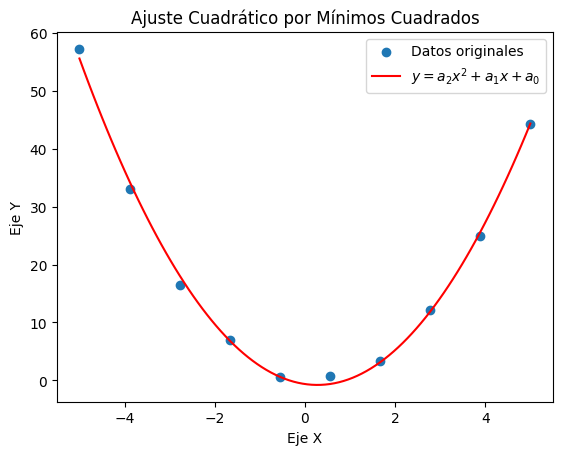
\includegraphics{determinante_files/figure-pdf/cell-6-output-2.png}




\end{document}
